\chapter{Phase Transitions and Critical Phenomena}
\label{ch:crit}

When trying to analyze a physical system, a big part of a physicist effort is
dedicated to identifying the parts that compose the system and how they
interact with each other. It is usually a daunting task to find an interaction
model that captures all the expected properties of a system. That's because the
macroscopic (i.e.\ collective) behavior does not follow trivially from the
microscopic forces in place. In no area of physics this is more clear than in
that of phase transitions and critical phenomena. Not surprisingly the
relationship between criticality and complexity has been applied to areas well
beyond the domain of atoms and molecules, like cognitive
sciences~\cite{Kello2010}, social scieces~\cite{Kron2009} and
ecology~\cite{Sole1999}, to name just a few.

But let's take a step back and look at the components that make up a physical
system. We can get away with making very little assumptions about their actual
identities. They can be elementary particles when studying high energy physics,
atoms and molecules when determining the electronic properties of a material,
living cells when observing the growing pattern of a colony of bacteria, or
even people when trying to design buildings with safe exit routes. What is more
important to us is the fact that these building blocks can organize themselves
in several different ways. Each pattern of organization is called a
\textit{phase}, and in which phase the systems finds itself depends on the
value of some external parameter, like energy density, temperature, nutrient
concentration or whether or not there's a fire in the building. Not only that
but different phases of a same system display wildly different macroscopic
behavior, despite no change taking place in their composition.

The most familiar example is water. At sea level, water is in its solid phase
for temperatures lower than $0^\circ$C. That happens because the water
molecules are locked in place by the cohesive forces that its neighbors exert
on each other. When the temperature is higher than $0^\circ$C but lower than
$100^\circ$C, the molecules acquire enough kinetic energy to be able to move
through one another. They still interact strongly enough to be bound together
but it is not sufficient to keep them fixed. This is the liquid phase. When the
temperature is above $100^\circ$C, water is now in the gaseous state, where
thermal movement starts dominating the dynamics of the system. The molecules
now move mostly unimpeded, interacting only when colliding directly. See
Fig.~\ref{fig:phases} for an illustration of how a molecule moves int the three
phases.

Not all phase transitions concern the states of matter.


\begin{figure}[h]
\begin{center}
    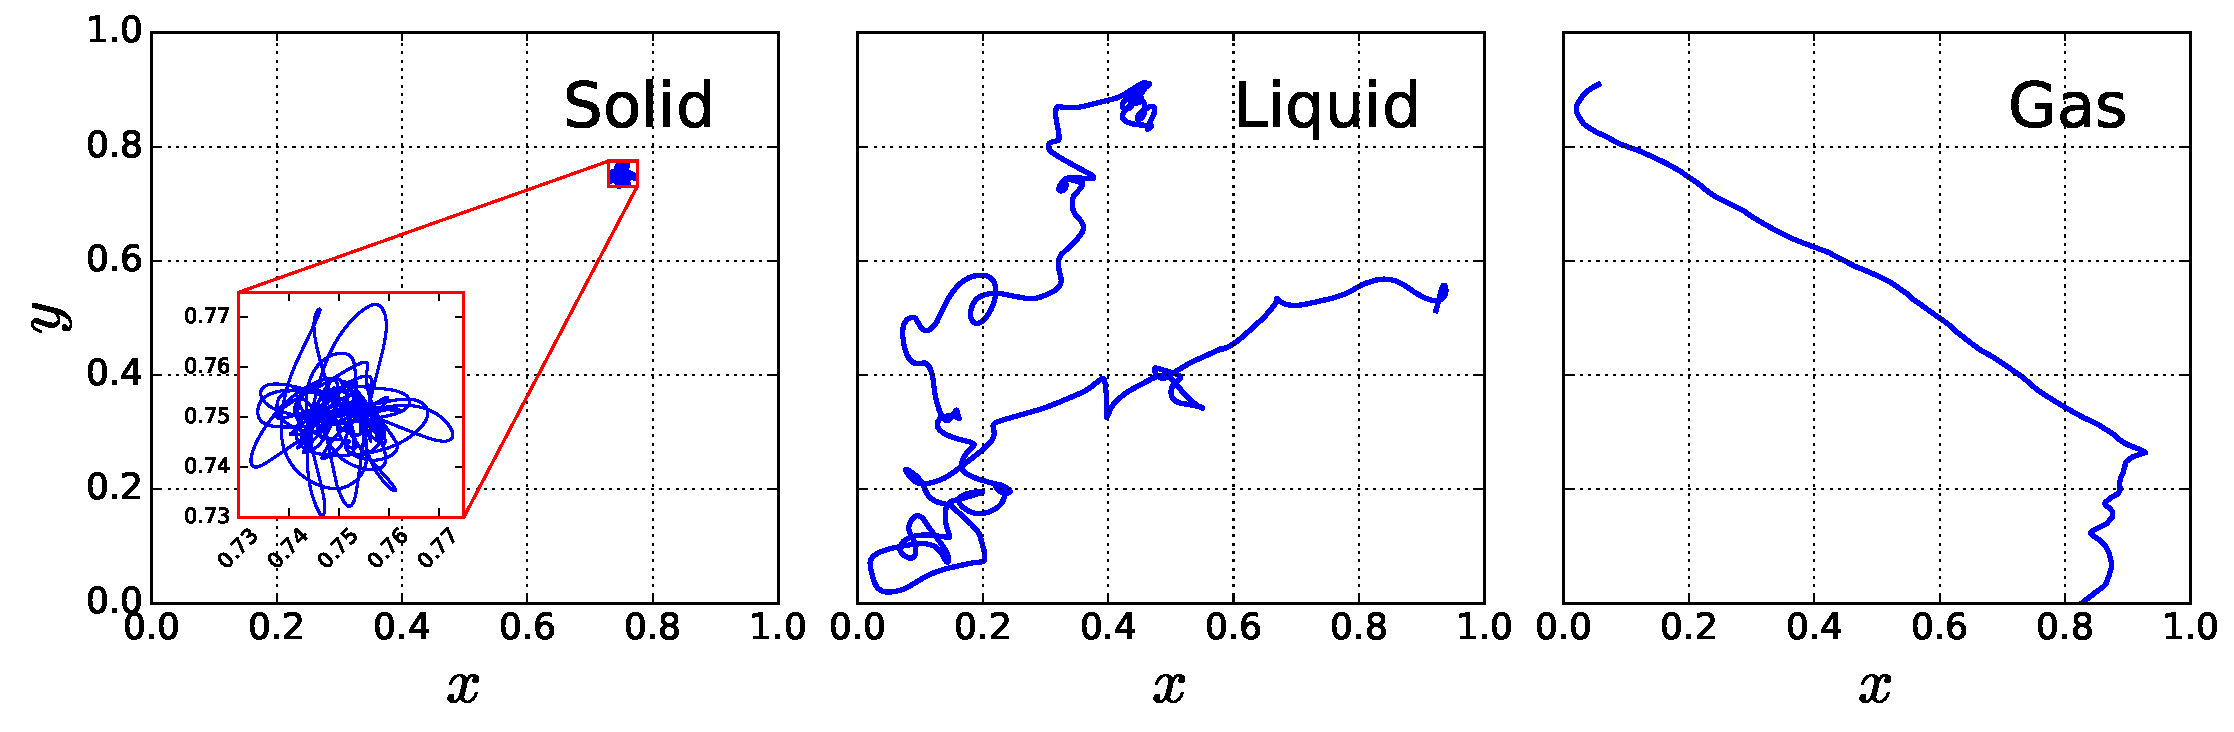
\includegraphics[scale=0.4]{chapters/ch2-crit/figs/phases}
\end{center}
\caption{How a system of particles behave in the three phases of matter. Here a
    simulation of 100 particles was done, but the trajectory of only one is
    shown. In the solid state the particles are confined to small region by
    the interactions of its neighbors. In the liquid state the particle is
    unconfined, but still interacts strongly with the other particles. In the
    gas state the kinetic energy of the particles is large enough that they
    barely interact with one another, making a ballistic trajectory until
    they make a head-on collision with another particle.}
\label{fig:phases}
\end{figure}


\begin{figure}[h]
\begin{center}
    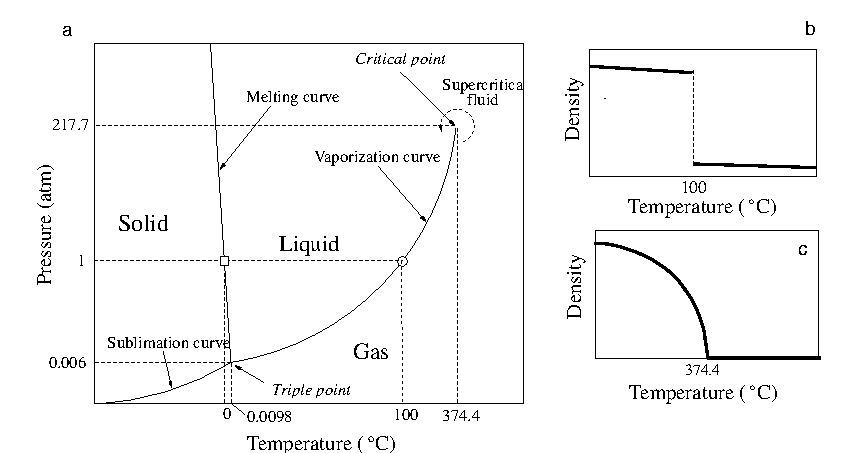
\includegraphics[scale=1.0]{chapters/ch2-crit/figs/water}
\end{center}
\caption{Phase diagram of water (a). Here, the three usual phases are
    distinguished, each separated from the other by a critical line. The phase
    transition that happens when the system traverse a line is characterized by
    a discontinuous jump in the density, as shown in (b) for the liquid-gas
    transition at $P=1$ atm. For $P=217.7$ atm however the same transition is
    continuous, as shown in (c). In the vicinity of this phase transition, at
    $T\approx374.4^\circ$C, the two phases become indistinguishable, and
    display a number of peculiarities. Systems in such state are called
    critical systems. Reproduced from~\cite{Sole2011}.}
\label{fig:water}
\end{figure}

